
\section{System Overview}

\begin{figure}
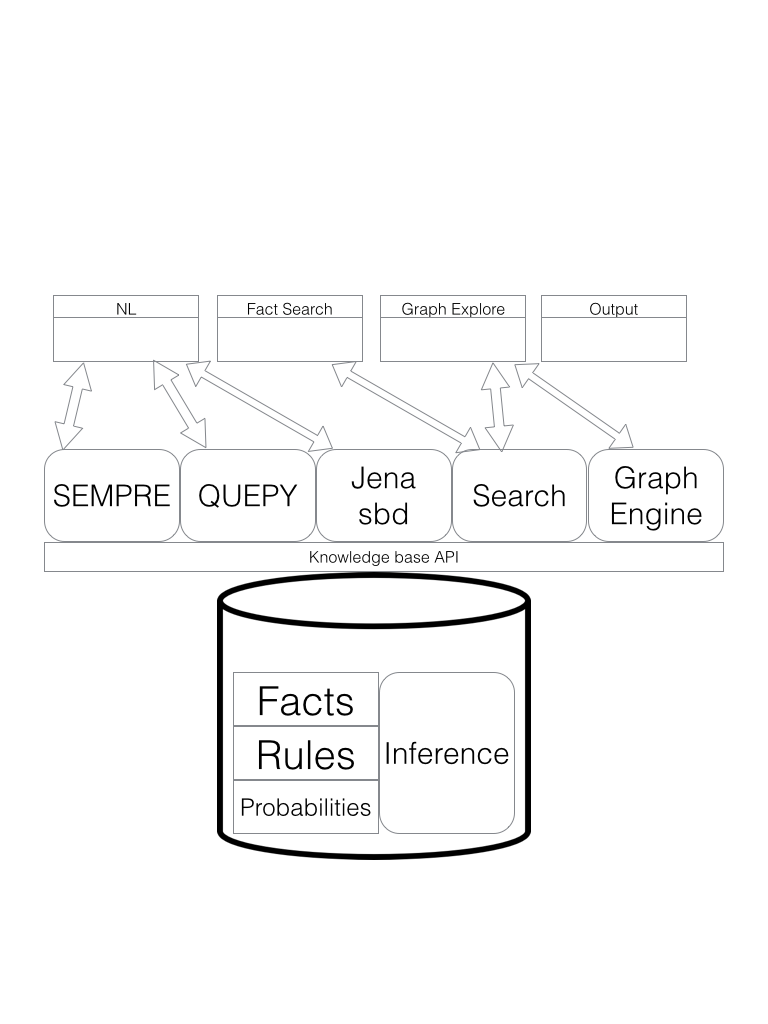
\includegraphics[width=\columnwidth,clip=true,trim=0cm 4cm 0cm 10cm]{images/qaarchitecture.png}
\caption{Question Answering system architecture.}
\label{fig:qaarchitecture}
\end{figure}



This demonstration describes a question answering systems designed around
a probabilistic knowledge base.
In this section, describe each component of the knowledge base system.
We begin with the interface, we describe each of the different methods
the users has to interact with with the backend knoweldge base.
We then describe the Logic layer that does translation and of user actions
to the back end actions. It also allows the user to see the current current
status of the system.
We also describe the probabilistic knowledge base driving the system.
We describe its schema and the integrated functions.



\subsection{Interface}

The framework is developed using AngularJS\@ to completely compatible with desktop and mobile devices.
The interface allows users to make queries using three different modalities.
Users will be able to enter natural language questions, search through the set of existing facts, and use a graph to explore connections between graphs.
New probabilistic facts and rules can also be added to the system through the interface.
Users can also remove or alter the existing facts and rerun queries.
The status of queries and the underlying processes are displayed on the main interface.


\subsubsection{Natural Language Interface}
Describe the purpose tranlation of natual language questions queries.
Add the auto complete for previous questions.

%QUEPY

%SEMPRE
We create a service that calls the SEMPRE 1.0 question answering system~\cite{berant2013freebase,berant2013semantic}.
This service takes a natural language questions matches against predicates aligned with Freebase.
We are then able to generate SPARQL queries to determine the answer of a query.



\subsubsection{Fact Search}
Describe how facts are searched using the database.
Describe how results are ranked.
Describe how new results are discovered.
\subsubsection{Graph Exploring}
Describe D3 visualization of graph and rule display
Describe user interaction with graph
Describe user selecting facts
Describe users removing facts


\subsection{Logic}
Describe the translation of NL-to-queries using templates (quepy) and also sempre.

Describe how rankings are computed from queries.
SEMPRE Returns probabilities, Quepy gives a 0 or 1 probability.
We compare the fact pobabilities to the sempre results.

\subsection{Knowledge Base}

Desscribe the PostgreSQL database and the other serices running on servers.
Describe the tables 
Describe the functions that are called
Describe the parallelism

The system is loaded with docker, a system container, so any modifications by demo can be quickly rolled back to the intial state.





% See other examples: http://www.vldb.org/2014/program/papers/demo/

